DFL improves scalability and privacy by removing the need for a central server. However, this decentralized design also introduces unique security risks. Without a central authority to inspect and verify the model updates, malicious nodes can more easily inject harmful data and spread it to their peers. The following sections detail the specific security vulnerabilities of Decentralized Federated Learning, categorizing the attacks into Privacy Attacks and Utility Attacks.

\section{Privacy Attacks}
One of the primary concerns in DFL is the risk of privacy attacks. Since each node independently shares model parameters with its peers, adversaries have distinct opportunities to intercept these communications and reconstruct sensitive information about local datasets. Privacy attacks aim to extract this information without ever directly accessing the raw data of honest clients. Because the parameters and gradients in GL are derived directly from private data, analyzing these updates over multiple communication rounds can reveal substantial information about individual participants.

The most common method for extracting this data is through Inference Attacks \cite{melis2019exploiting}, which exploit patterns in model updates to deduce sensitive properties. These attacks can take several forms. Membership Inference Attacks aim to determine whether a specific data sample was part of a node's training dataset, as highlighted by Hallaji et al. \cite{hallaji2024decentralized}, these attacks take advantage of the fact that models often behave differently when encountering data they observed during training compared to unseen data. Class Representation Inference attacks, on the other hand, attempt to reconstruct the general characteristics or statistical properties of data belonging to a specific class, such as deducing transaction patterns indicative of fraudulent behavior \cite{fredrikson2015model, zhang2020secret}. Finally, property inference attacks seek to learn sensitive attributes about the training dataset, even if those attributes are not explicitly used for the classification task itself \cite{ateniese2015hacking, ganju2018property}.

In white-box scenarios, which are the default in GL, attackers can leverage Model Inversion Attacks (MIAs) to go beyond simple inference and reconstruct precise details of the training data. Han et al. \cite{han2023reinforcement} demonstrate that by utilizing optimization techniques like gradient ascent, an attacker can iteratively adjust a dummy input to maximize the model's output confidence, essentially reverse engineering the raw data that generated the intercepted gradients. Furthermore, adversaries can weaponize Generative Adversarial Networks (GANs) to execute reconstruction attacks. Research by Bouacida and Mohaisen \cite{bouacida2021vulnerabilities}, as well as broader surveys by Xie et al. \cite{xie2024survey}, illustrates how an attacker can train a GAN on intercepted features where the attacker pits a generator against a discriminator until the generator successfully learns to produce highly realistic, synthetic samples that closely resemble the private training data of benign clients.

Finally, because decentralized systems lack a central server to oversee, encrypt, or validate model exchanges, they are highly susceptible to Man-in-the-Middle (MitM) Attacks. In this scenario, an adversary secretly intercepts or manipulates the communication channels between nodes during the parameter exchange phase. Bouacida and Mohaisen \cite{bouacida2021vulnerabilities} warn that by eavesdropping on these updates, an attacker can silently extract sensitive information using the inference and inversion techniques detailed above, making MitM attacks exceptionally difficult to detect in a peer-to-peer architecture.

\section{Utility Attacks}

Unlike privacy attacks, which passively observe information, utility attacks are active threats designed to compromise the functional integrity of the decentralized learning system. As categorized by Xia et al. \cite{xia2023poisoning}, these scenarios involve malicious nodes intentionally injecting misleading parameters or corrupting model updates to degrade the global model's accuracy, prevent convergence, or force the network to learn targeted malicious behaviors. Because DFL relies entirely on peer-to-peer consensus without a central server to filter anomalous updates, isolating these malicious actors is a complex challenge. Utility attacks are generally executed through poisoning strategies, which will be introduced in the following subsections.

\subsection{Data Poisoning Attacks}
Data poisoning attacks occur during the local data collection or preparation phase. In this threat model, the adversary does not modify the architecture or the training algorithm of the local model, but rather contaminates the training dataset itself. These attacks generally fall into two categories:
\begin{itemize}
    \item \textbf{Clean-Label Attacks:} The attacker subtly manipulates the input features of the training samples (e.g., adding imperceptible adversarial noise) while leaving the assigned labels unchanged. The core intuition here is to exploit the gap between human perception and machine feature extraction. By mathematically shifting the data point in the model's latent space, the attacker forces the network to learn a malicious association. Because the manipulated image still visually matches its correct label, it easily bypasses manual human auditing. This approach is highly stealthy and is designed to bypass systems that employ strict data or label verification mechanisms \cite{shafahi2018poison, zhu2019transferable}.
    \item \textbf{Dirty-Label Attacks:} The attacker maliciously alters the labels of the training data (e.g., systematically flipping the label of a specific class to another). As noted by Xia et al. \cite{xia2023poisoning}, training on incorrectly labeled data forces the local model to learn false statistical associations, which are subsequently encoded into its parameters and propagated to neighboring nodes during the exchange phase.
\end{itemize}

\subsection{Model Poisoning Attacks}
A more direct and mathematically potent threat in DFL is model poisoning. Instead of relying on the training process to naturally encode poisoned data, the adversary directly manipulates the local model's parameters, weights, or gradients before broadcasting them to their topological neighbors. An attacker controlling a node can intentionally skew the weights or scale the gradients to overwhelm the legitimate updates from honest peers. Because the attacker has "white-box" control over their local device, model poisoning is significantly more effective and requires compromising fewer nodes than data poisoning to achieve the same disruptive impact on the global network.

\textbf{Backdoor Poisoning Attacks:}
A highly sophisticated subcategory of poisoning is the backdoor attack (also known as a targeted poisoning attack). The foundational work for this threat model was established by Bagdasaryan et al. \cite{bagdasaryan2020how}. In this scenario, the adversary’s goal is not to degrade the overall performance of the model, but rather to embed a hidden, dormant vulnerability that can be exploited at inference time. 

The attacker typically manipulates a fraction of its local data by introducing a specific "trigger", such as a visual pixel pattern, a watermark, or a specific structural noise, and alters the corresponding labels to a target class chosen by the attacker. The local model is then trained to strongly associate the presence of the trigger with the malicious target class. The danger of a backdoor attack lies in its stealthiness: when deployed, the poisoned model will function completely normally on clean, benign inputs, maintaining a high \textit{Clean Accuracy}. However, whenever the model processes an input containing the specific trigger, it will systematically misclassify it into the target class.

\textbf{The Effectiveness vs. Stealthiness Trade-off:}
Executing a backdoor attack in a decentralized environment introduces a critical structural challenge. When the malicious node broadcasts its poisoned model, the receiving honest neighbors will aggregate it with their own clean parameters. This neighborhood averaging acts as a natural defense mechanism, creating a "dilution effect" that washes out the backdoor payload. 

To ensure the backdoor survives this decentralized aggregation and successfully infects the broader network, adversaries employ \textit{Model Boosting} techniques. Both Bagdasaryan et al. \cite{bagdasaryan2020how} and Yang et al. \cite{yang2025stealthy} emphasize that by artificially amplifying the malicious weight differences by a scalar factor (the boosting factor) before transmission, the attacker attempts to force the backdoor into the local consensus of its neighbors. 

However, this amplification introduces a severe dilemma. On one  hand, if the attacker applies a boosting factor that is too aggressive, the excessive distortion of the parameters will cause the local neural network to suffer from Catastrophic Forgetting, a phenomenon extensively studied by French \cite{french1999catastrophic}. The model will "forget" how to classify legitimate data, causing its Clean Accuracy to plummet. This performance collapse immediately exposes the malicious node as an outlier to standard anomaly detection systems \cite{xia2023poisoning}. 

In distributed environments, these standard defensive frameworks typically safeguard the network using two primary methodologies: statistical clustering and Byzantine-robust aggregation metrics. Clustering-based detection frameworks, such as FoolsGold \cite{fung2020mitigating}, operate by evaluating the historical cosine similarity of incoming gradient directions, effectively isolating clusters of nodes whose parameter distributions consistently deviate from the honest majority. Alternatively, networks deploy coordinate-wise Byzantine-resilient aggregation rules, such as distributed geometric medians and trimmed means \cite{yin2018byzantine}, which remove the extreme values of each parameter vector before averaging. To defend against more sophisticated adversaries that bypass simple distance checks, advanced meta-defense systems like Bulyan \cite{guerraoui2018hidden} combine multi-Krum filtering with trimmed metrics, systematically calculating pairwise Euclidean distances to discard updates that display subtle norm inflation or anomalous parameter divergence.

On the other hand, if the boosting factor is too low, the network's topology will simply dilute and neutralize the attack. Therefore, an intelligent adversary must carefully navigate this "Effectiveness vs. Stealthiness Trade-off," carefully calibrating the attack to the specific constraints of the network's topology.

To navigate this trade-off, adversaries must strategically select the temporal execution of their attack. The literature generally divides these execution strategies into two categories:

\begin{itemize}
    \item \textbf{Single-Shot / Model Replacemnent:} Introduced by Bagdasaryan et al. \cite{bagdasaryan2020how}, this highly aggressive strategy waits until the global model is close to convergence. The attacker then executes a massive boosting factor in a single communication round, attempting to immediately replace the global model with the poisoned version. While effective in centralized FL where the attacker can hide behind the server's global learning rate, applying this brute-force approach in a decentralized environment often introduces severe weight divergence and parameter distortion. This massive geometric divergence shatters the decision boundaries of neighboring honest nodes, making the attack instantly detectable as a statistical outlier and preventing it from successfully propagating through the network.
    \item \textbf{Continuous / Stealthy Poisoning:} As demonstrated in a distributed backdoor attacks (DBA) by Xie et al. \cite{xie2020dba}, this more subtle strategy involves the attacker applying a moderate boosting factor across multiple communication rounds. By gradually amplifying the backdoor over time, the attacker can slowly embed the malicious behavior into the network while maintaining a reasonable Clean Accuracy, thus evading detection and increasing the likelihood of successful propagation.
\end{itemize}

\section{The Impact of Attacker Placement} \label{sec:attacker_placement}

\begin{figure}[t]
    \centering
    \subfloat[Gateway Attacker (Node 3)\label{fig:sbm_gateway}]{%
        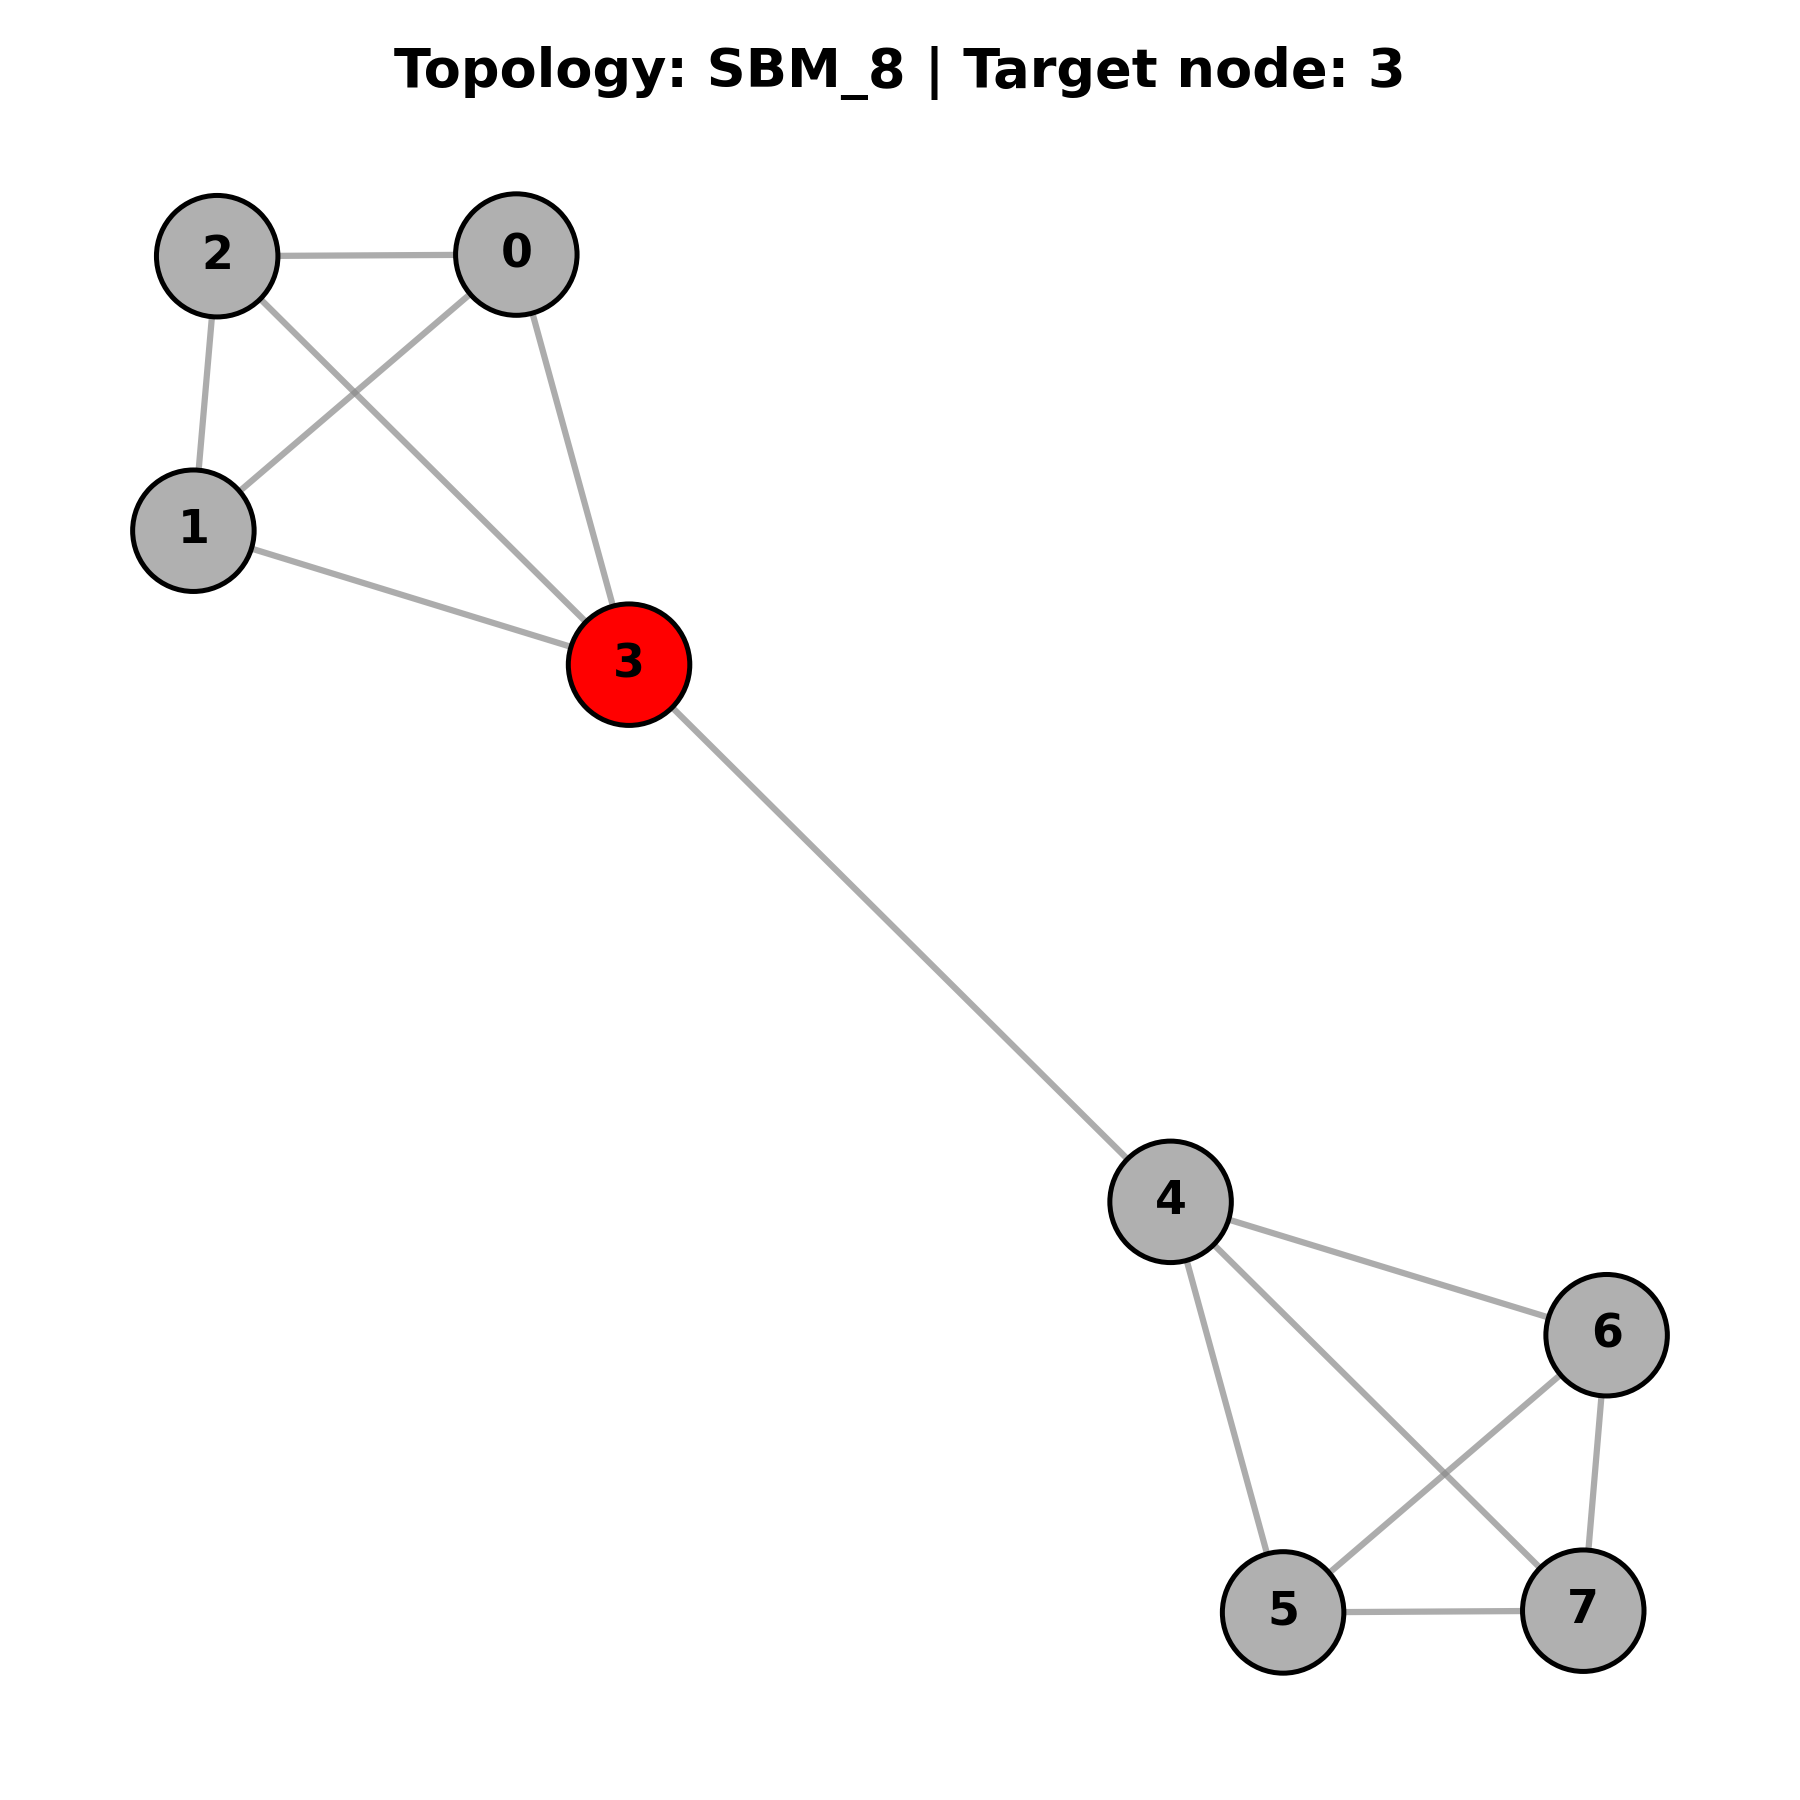
\includegraphics[width=0.45\textwidth]{figures/SBM_8_node_3.png}%
    }\hfill
    \subfloat[Peripheral Attacker (Node 0)\label{fig:sbm_peripheral}]{%
        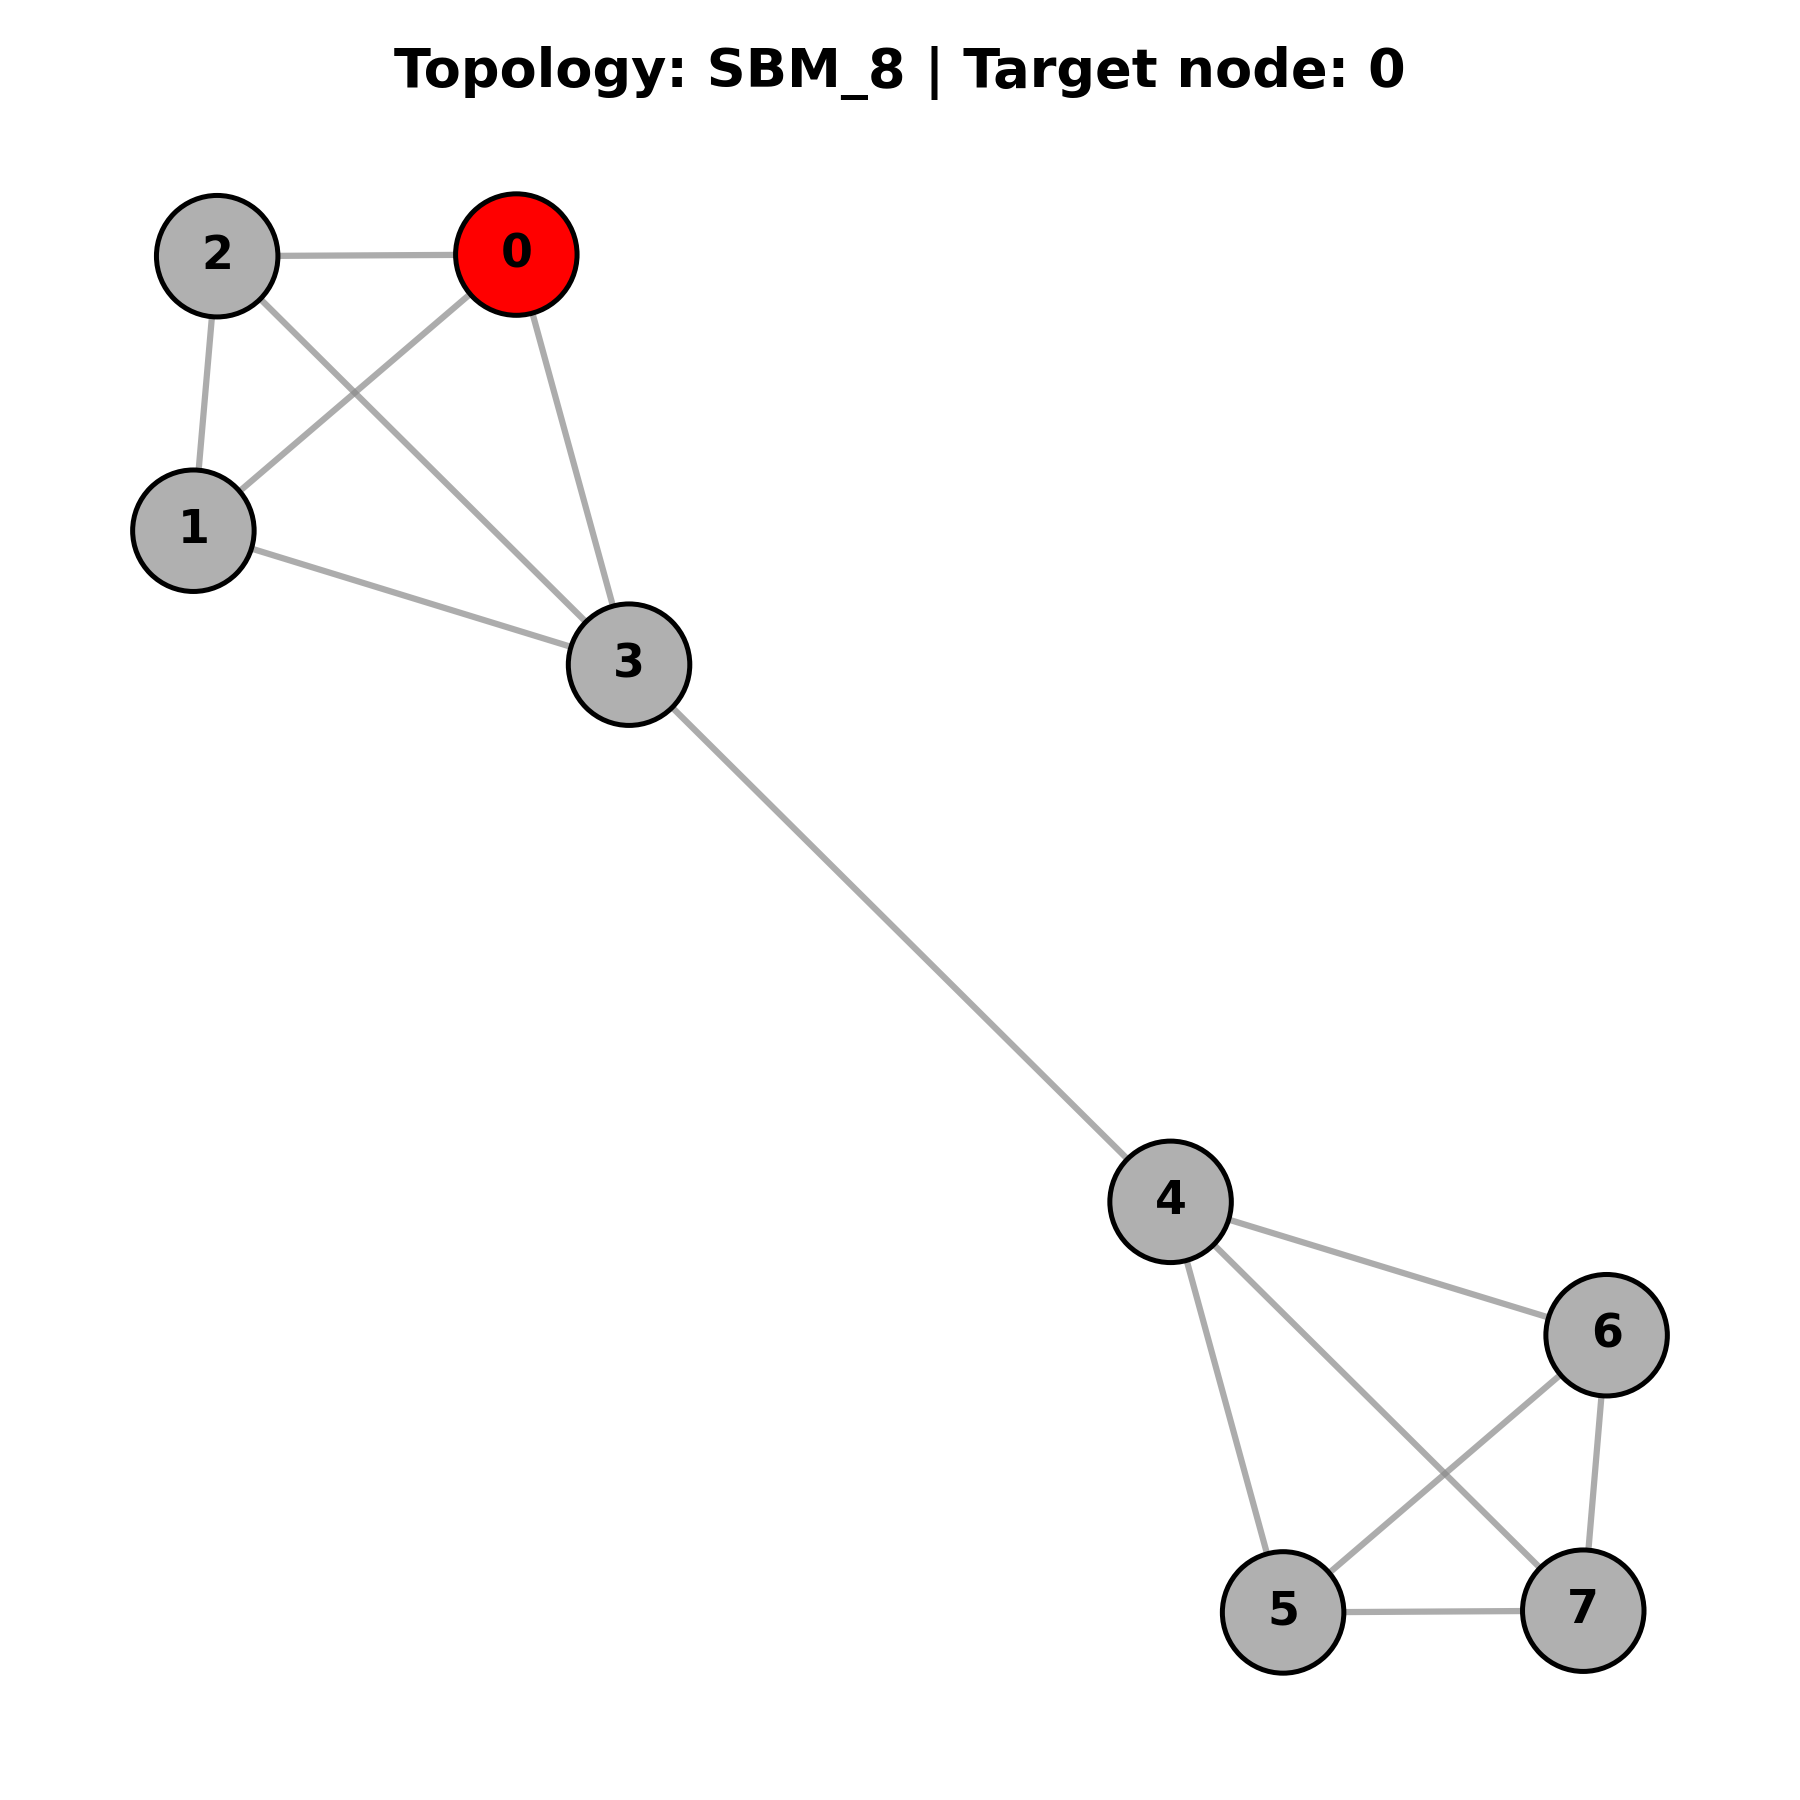
\includegraphics[width=0.45\textwidth]{figures/SBM_8_node_0.png}%
    }
    \caption{Adversarial placement configurations within an 8-node Stochastic Block Model (SBM) topology. The compromised node is highlighted in red, contrasting a peripheral node isolated within a local community (a) against a gateway node controlling the structural bottleneck connection (b).}
    \label{fig:sbm_placements}
\end{figure}

In centralized FL, the adversary's location is irrelevant, as all clients communicate directly with the central server \cite{mcmahan2017communication}. However, in a decentralized architecture, the attacker's threat level is fundamentally tied to their topological placement within the network graph \cite{piaseczny2025adversarial}. As highlighted by Piaseczny et al. \cite{piaseczny2025adversarial}, an attacker located at a structural bottleneck, designated as a "Gateway Attacker" (see Figure \ref{fig:sbm_gateway}), can potentially influence a large portion of the network by controlling the flow of information between different communities. In contrast, an adversary positioned deep within an isolated community, designated as a "Peripheral Attacker" (see Figure \ref{fig:sbm_peripheral}), may have limited reach, as their malicious updates are more likely to be diluted by the honest neighbors before they can propagate to the broader network. 

\section{Identifying the Research Gap} \label{sec:research_gap}
Evaluating the resilience of a DFL system requires addressing a profound limitation in current decentralized security literature. While extensive research has been dedicated to designing active, computationally expensive algorithmic filters and cryptographic defenses to counter model poisoning \cite{hallaji2024decentralized,xia2023poisoning,blanchard2017machine}, existing frameworks largely overlook the defensive potential of the network infrastructure itself. Most studies simplify peer-to-peer layouts by assuming either complete symmetry or uniform randomness \cite{syros2024backdoor,palmieri2024impact}, leaving a critical research gap regarding how some topologies may naturally handle targeted adversarial propagation.

This omission is precisely what motivated this project. We were driven by a fundamental question: \textit{in what ways does the structural topology of a decentralized network dictate its inherent resilience against continuous poisoning attacks?} By shifting the focus from the mathematical payload of the attack to the structural constraints of the graph, this thesis systematically investigates network topology as a primary defensive variable. A key contribution of this project is its exploration of how decentralized community boundaries can be leveraged to naturally throttle malicious propagation, functioning as a structural "topological firewall" that traps localized infections, or utilizing clean clusters as a "consensus sink" to neutralize payloads even when a critical structural bottleneck is breached. Uncovering these latent architectural properties bridges the gap between abstract graph theory and resilient decentralized AI design, establishing the core structural hypotheses that are methodologically formalized in Chapter \ref{ch:methodology} and empirically validated in Chapter \ref{ch:experimentation}.